\chapter{Model Specification}
\label{chap:1} 
In this chapter we describe the abstract models used to shape all the three parts of the system. (FARE QUI UN ELENCO? torretta, puntamento, kobuki)
\section{Turret Model}
Degree of Freedom (DoF) is the number of independent parameters that define the configuration of a mechanical system. In our case, we wanted to build a two DoF Pan \& Tilt turret. That means that our parameters are two angles. In a 3D reference system, \textbf{pan} is the horizontal angle about the upright Z axis, \textbf{tilt} is the vertical angle about the rotated Y axis. FIGURA PER MOSTRARE PAN AND TILT
Our final goal is to be able to define the direction of a laser ray mounted on top of the turret, so that we can control the position of the projected laser dot on a given surface, by solving the system's inverse kinematics.\\

For those purposes, we have built two different turrets. Since the model of the first one is slightly simpler than the second, we will start describing the former, which turns out to be helpful to understand the latter. We will focus on the case in which the laser must be projected on the ground.

\subsection{First Model}\label{subs:firstModel}
First, figure \ref{fig:firstModelRefFrame} helps us understand how we have shaped the model to match the physical structure of the turret. We have three reference frames. The \textbf{base\_frame} is fixed and is the one in which we define the coordinates of the projected point. \textbf{pan\_frame} and \textbf{tilt\_frame} are the frames used to represent our revolute joints.
\textbf{H} is the height of the turret, which is known. Note that the convention used for the frame is the following:
\begin{itemize}
    \item red is the x axis;
    \item green is the y axis;
    \item blue is the z axis.
\end{itemize}
Thus, we consider the laser ray to be a prolongation of the x axis of the \textbf{tilt\_frame}. \\
Figure \ref{fig:firstModelPanTilt} shows what we want to be able to do: given the \textit{x}, \textit{y} and \textit{z} of the laser point we want to set \textbf{pan} and \textbf{tilt} angles accordingly. In order to do so, firstly we will solve the forward kinematic, then the inverse will be easily derived.
\subsubsection{Forward Kinematic}
The forward kinematic should take as input our parameters (i.e. \textbf{pan} and \textbf{tilt}) and then return the coordinates of the laser projected point into \textbf{base\_frame} reference. 
Note that, since we are controlling the direction of an infinite ray, in order to obtain a unique (\textit{x, y, z}) triple, we must intersect such ray with a plane defined by the triple (\textit{0, 0, z}). In the forward kinematic equations this can be obtained by assuming that we know the \textit{z} of the point we want. Another option could be to assume that \textit{z} is zero, since we are considering the laser projection on the floor (i.e. on the \textbf{base\_frame}). \\
As well as what is already defined in figure \ref{fig:firstModelPanTilt}, we must add:
\begin{itemize}
    \item \textbf{L} as the distance from the \textbf{pan\_frame} origin to the projection of the laser point on the \textbf{base\_frame};
    \item \textbf{D} as the distance from the \textbf{tilt\_frame} origin to the laser point.
\end{itemize}
First, note that the \textbf{pan} angle does not depends on the \textit{z} coordinate, so, starting from:
\begin{align}
	D=& \frac{H-z}{\cos{(tilt)}} \label{eq:d}\\
	L=& \sqrt{(H-z)^2 + D^2}
\end{align}
We can easily obtain laser point coordinates:
\begin{align}
	x=& L\cos{(pan)}\label{eq:x}\\
	y=& L\sin{(pan)} \label{eq:y}
\end{align}

\begin{figure}
	\centering
	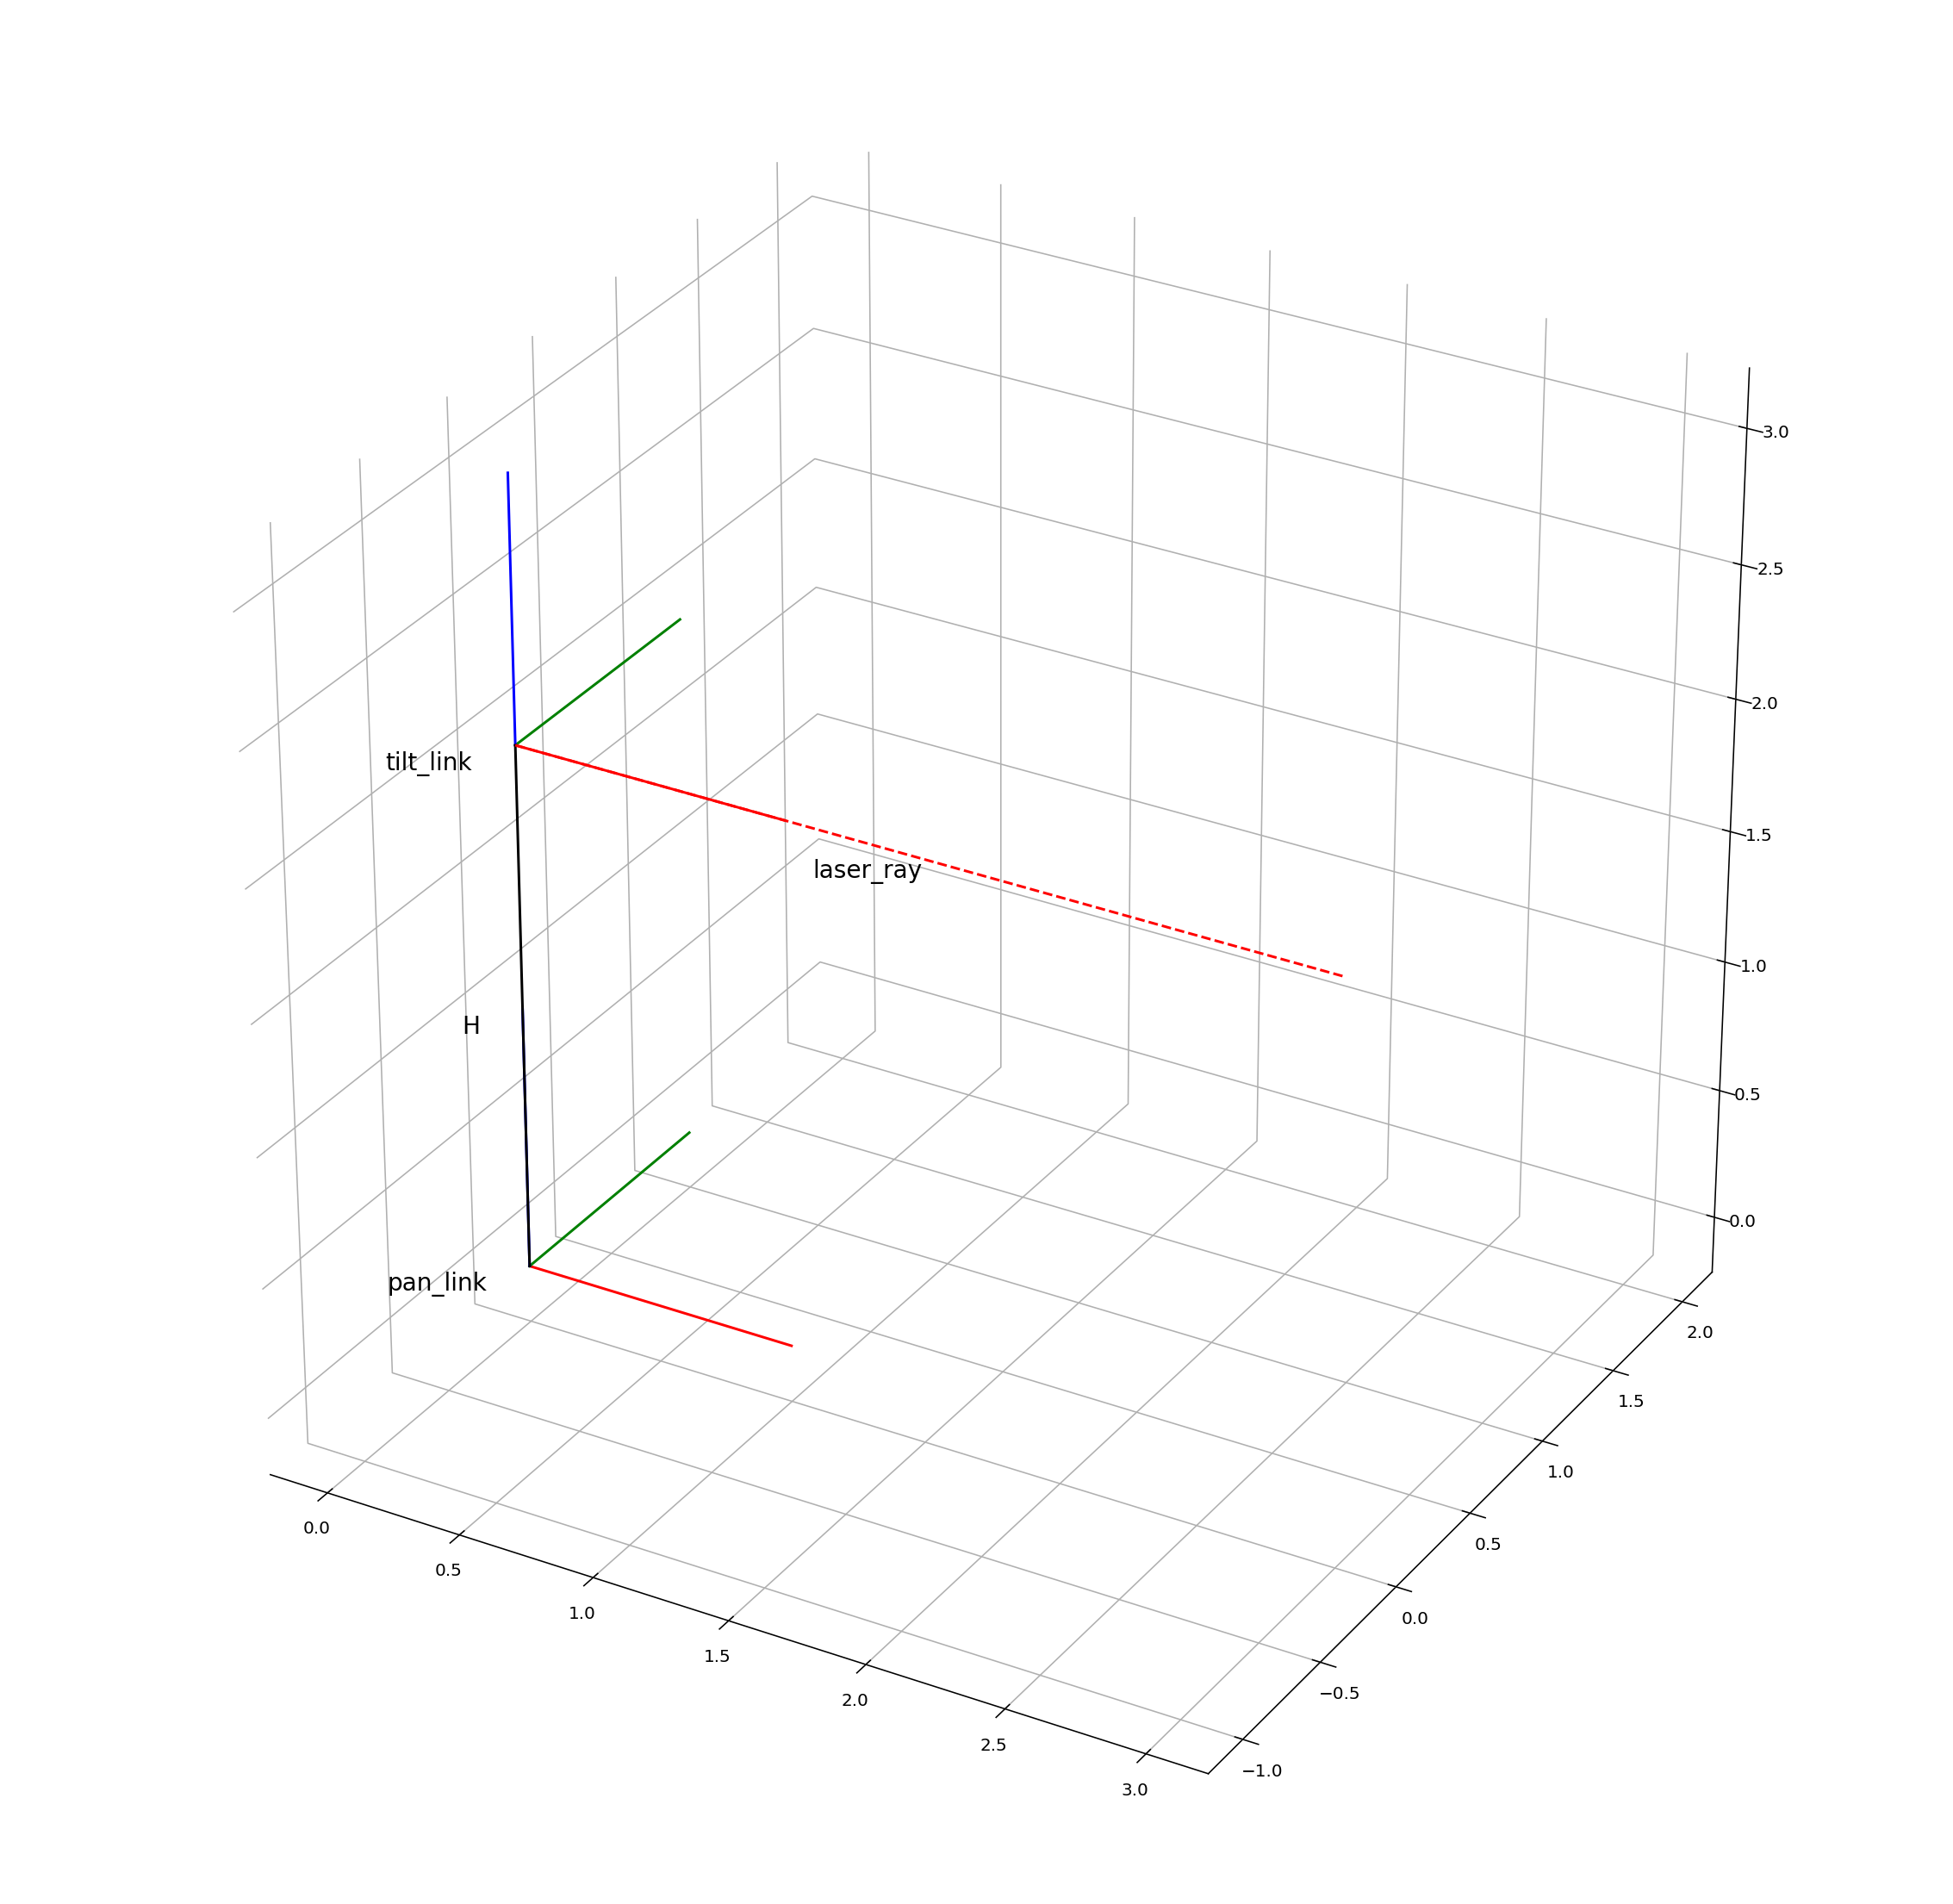
\includegraphics[width=\textwidth]{img/firstModel.png}%
	\caption{First Model, Reference Frames}
	\label{fig:firstModelRefFrame}
\end{figure}
\begin{figure}
	\centering
	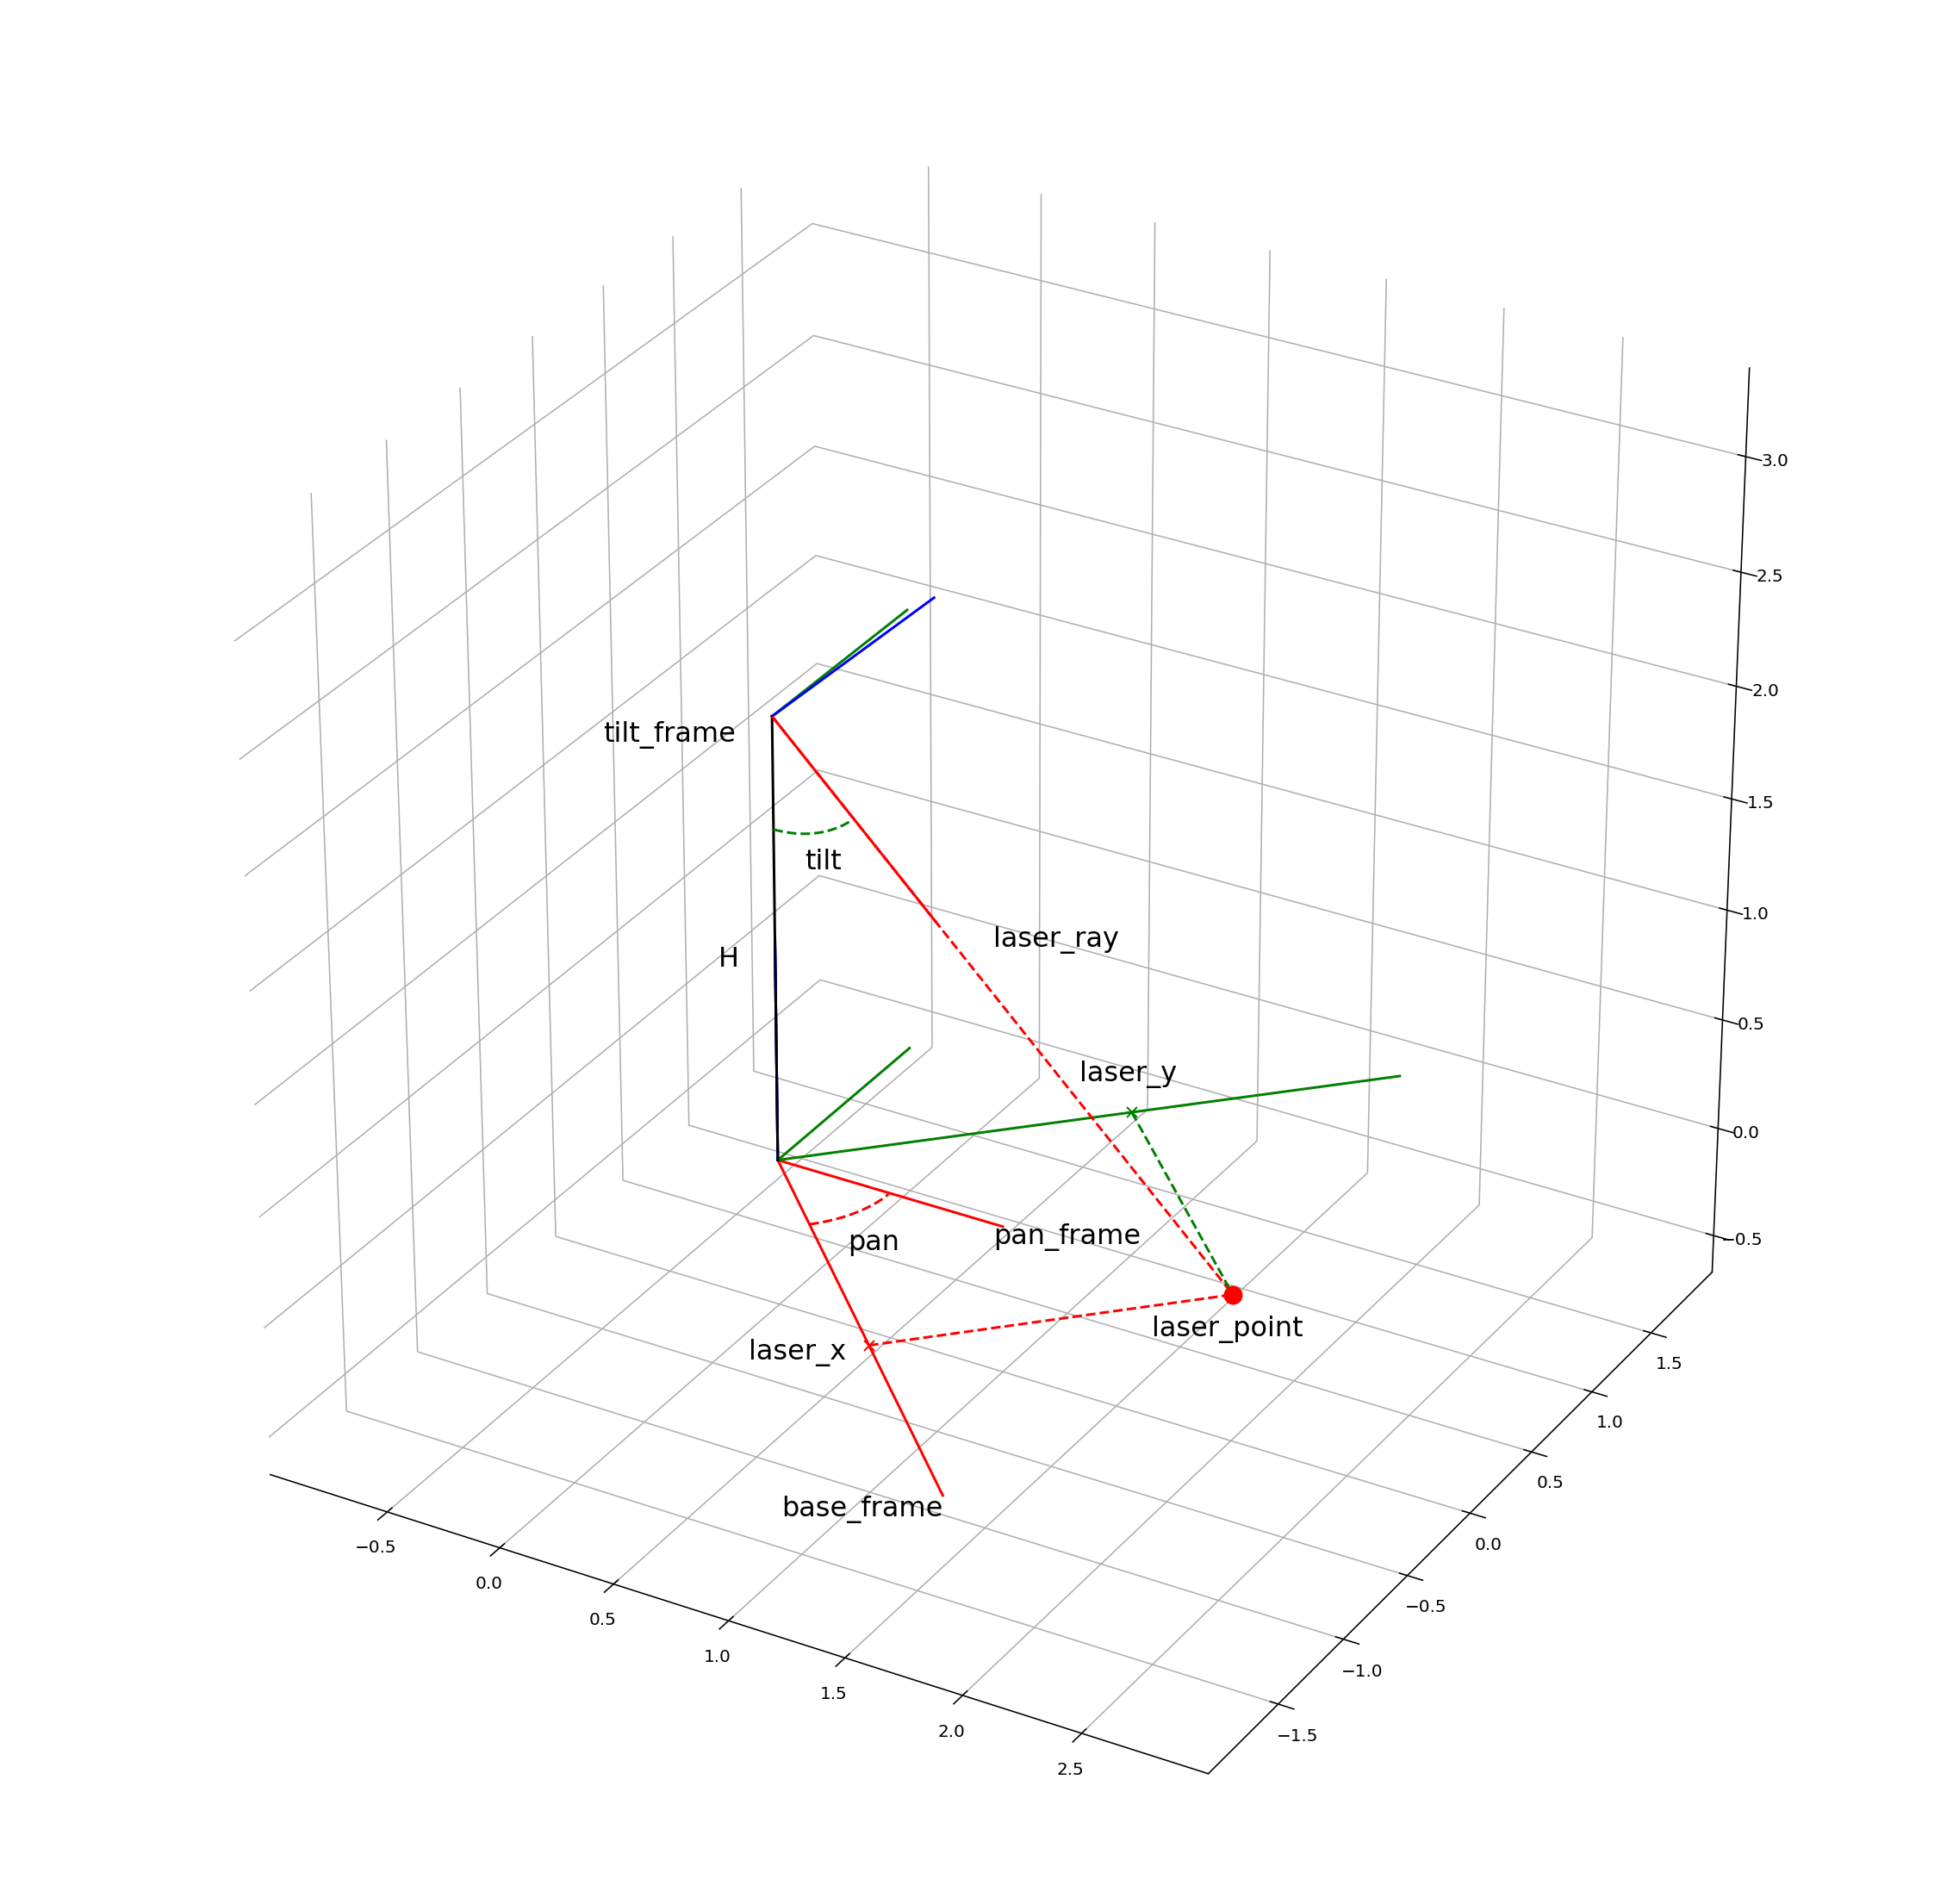
\includegraphics[width=\textwidth]{img/model1XY.png}%
	\caption{First Model, Pan \& Tilt Angle}
	\label{fig:firstModelPanTilt}
\end{figure}
\subsubsection{Inverse Kinematic}
The inverse kinematic takes as input the triple (\textit{x, y, z}) of the laser point and returns the corresponding \textbf{pan} and \textbf{tilt} angles.\\
In addition to \ref{eq:d}, we can say that:
\begin{align}
    H-z =& D\by\cos(tilt)\\
	L =& D\by\sin(tilt) \label{eq:dsin}\\
	L=& \sqrt{x^2+y^2}
\end{align}
Thus, we have that:
\begin{align}
    tilt =& \arctan\bigg(\frac{L}{H-z}\bigg) \label{eq:tiltik}\\
\end{align}
Finally, thanks to equations \ref{eq:x} and \ref{eq:y} we can immediately obtain:
\begin{align}
	pan=& \arctan\bigg(\frac{y}{x}\bigg)\label{eq:panik}
\end{align}
\\
\subsection{Second Model}
The second model is slightly different from the first, as we can see in figure \ref{fig:secondModelRefFrame}. In that case, we have the laser ray which is perpendicular to the x axis of the \textbf{tilt\_frame}. One could think that to solve the inverse kinematic, adding 90 degrees to the tilt angle could be enough. However, since the ray origin does not coincide with the origin of the frame, this is wrong. Changing the tilt angle will not change only the direction of the ray, but also the position of its origin. This makes the kinematic a bit more complicated for that model.
\\
Here we report only the inverse kinematic as it is the most interesting to understand. Note that the assumption made for the \textit{z} of the laser point in section \ref{subs:firstModel} still holds.

\begin{figure}
	\centering
	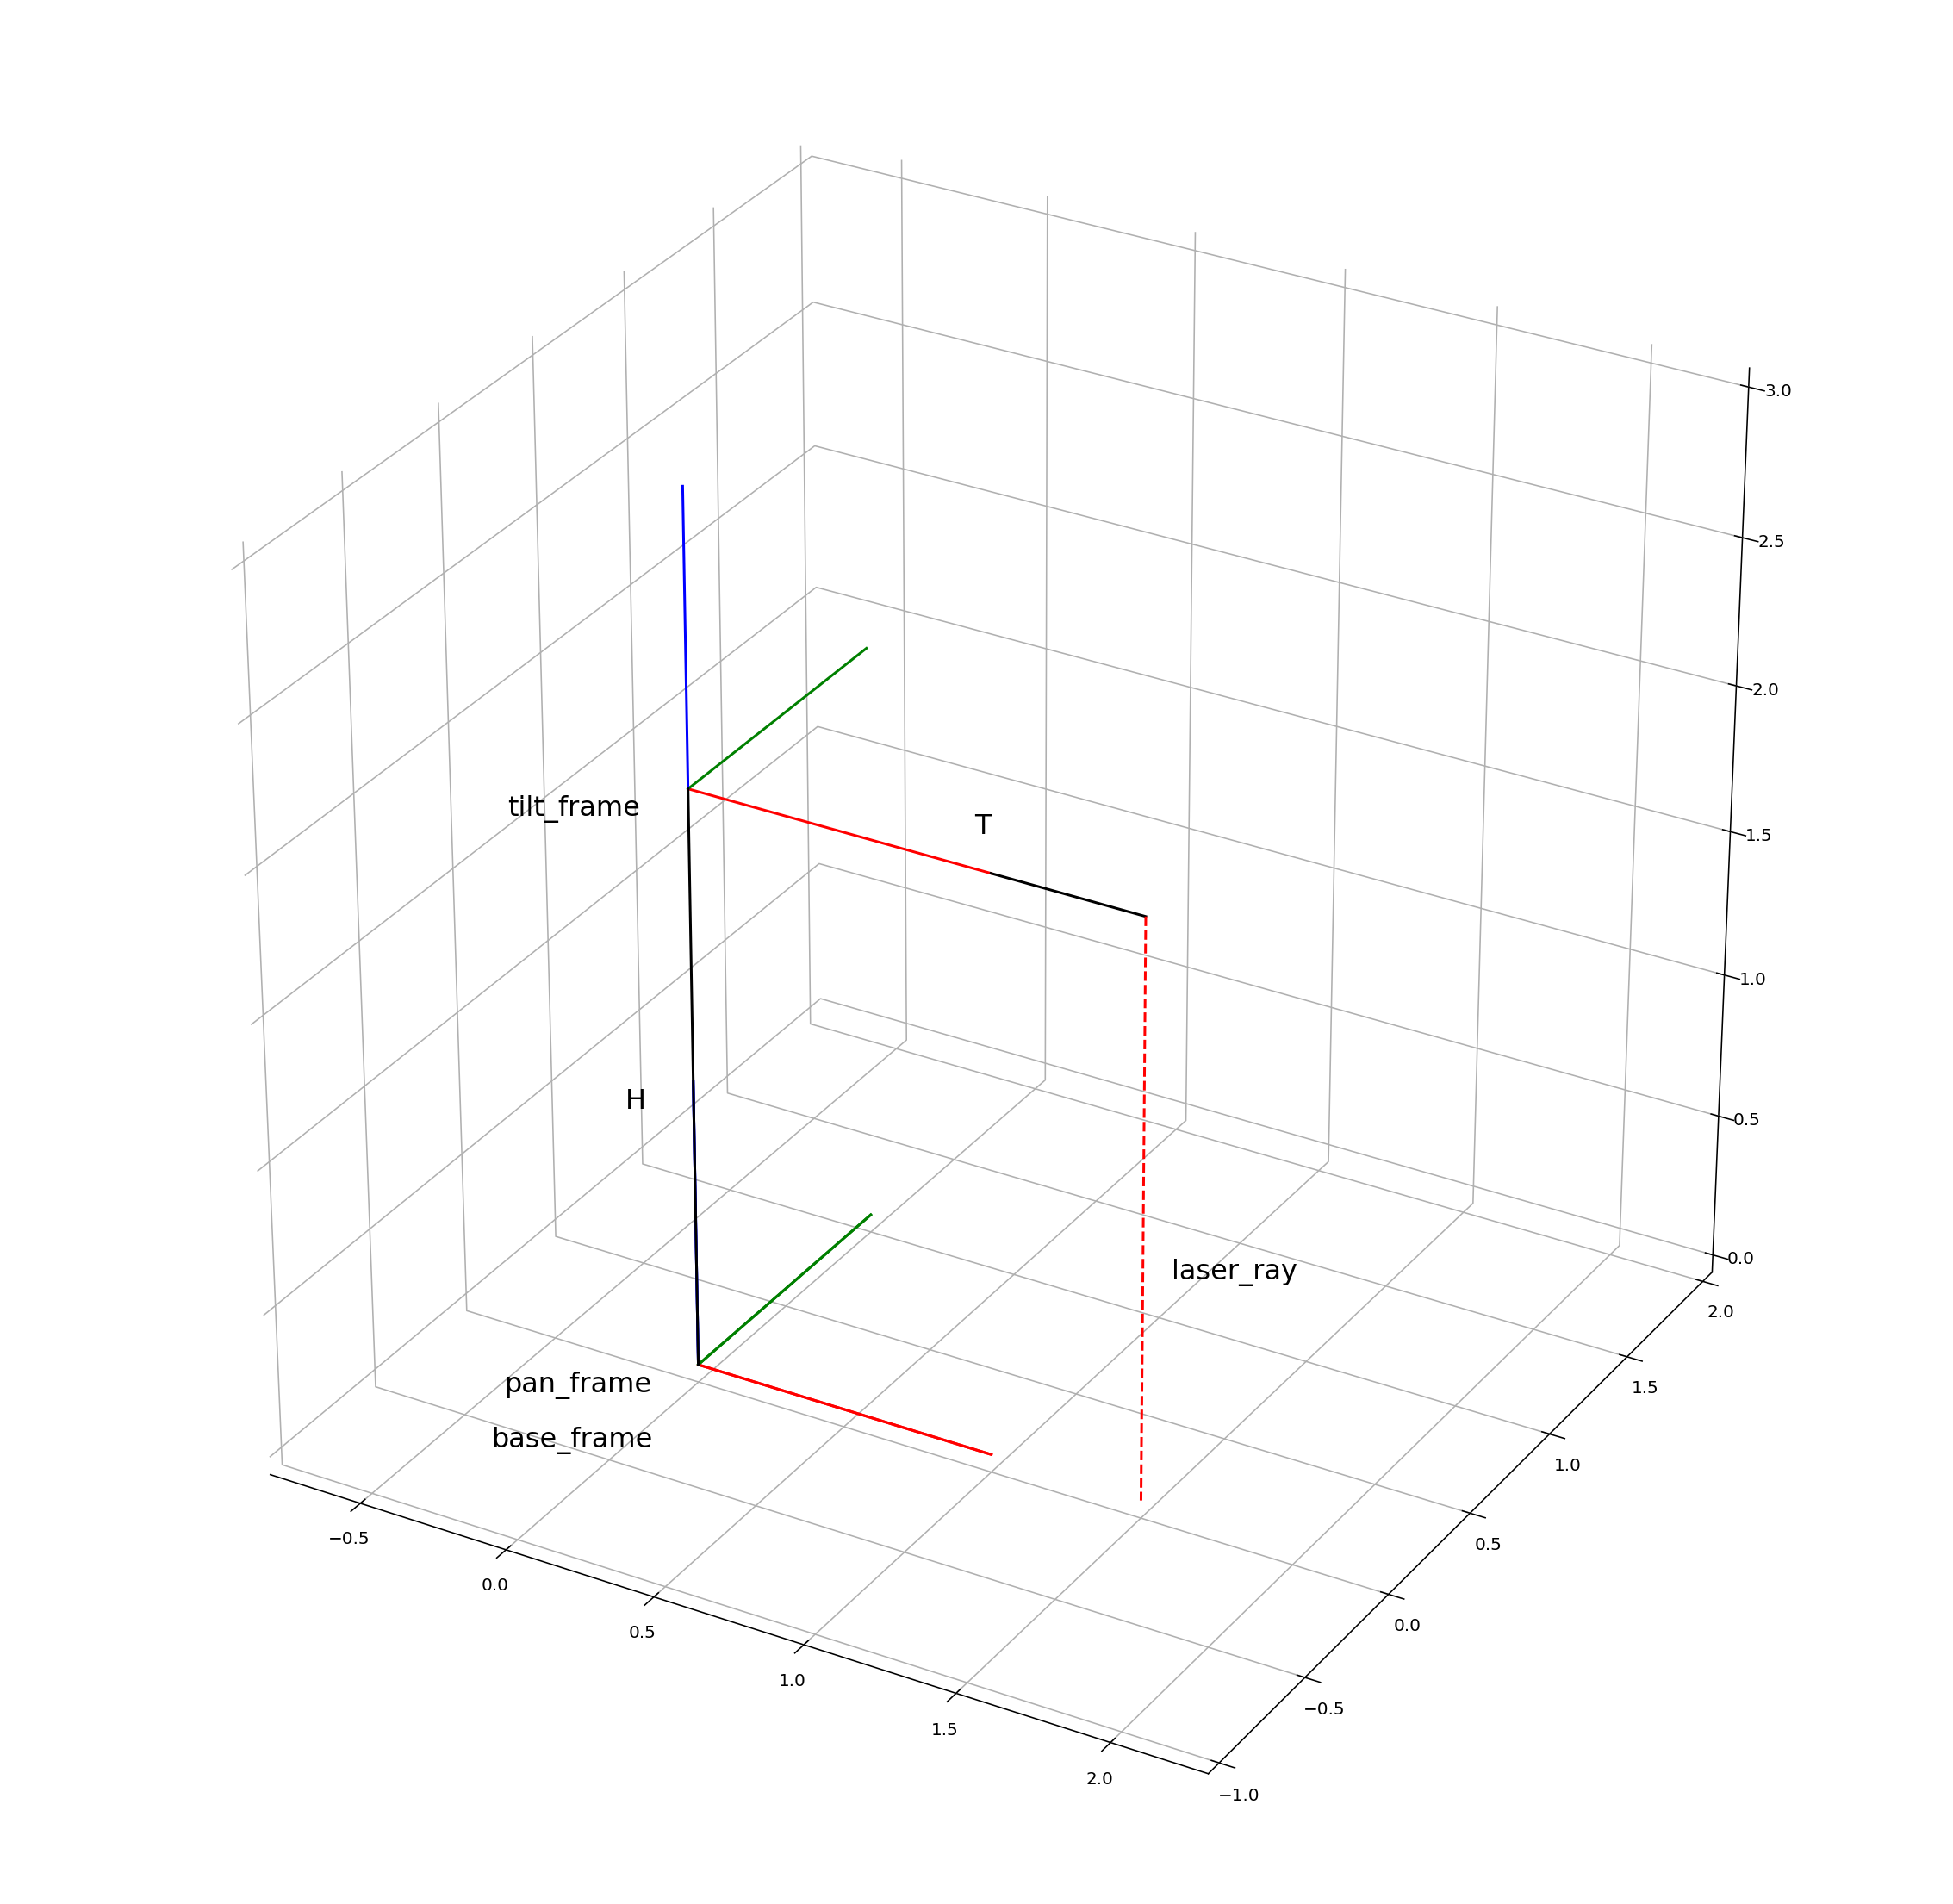
\includegraphics[width=\textwidth]{img/secondModel.png}%
	\caption{Second Model, Reference Frames}
	\label{fig:secondModelRefFrame}
\end{figure}

\subsubsection{Inverse Kinematic}
\begin{figure}
	\centering
	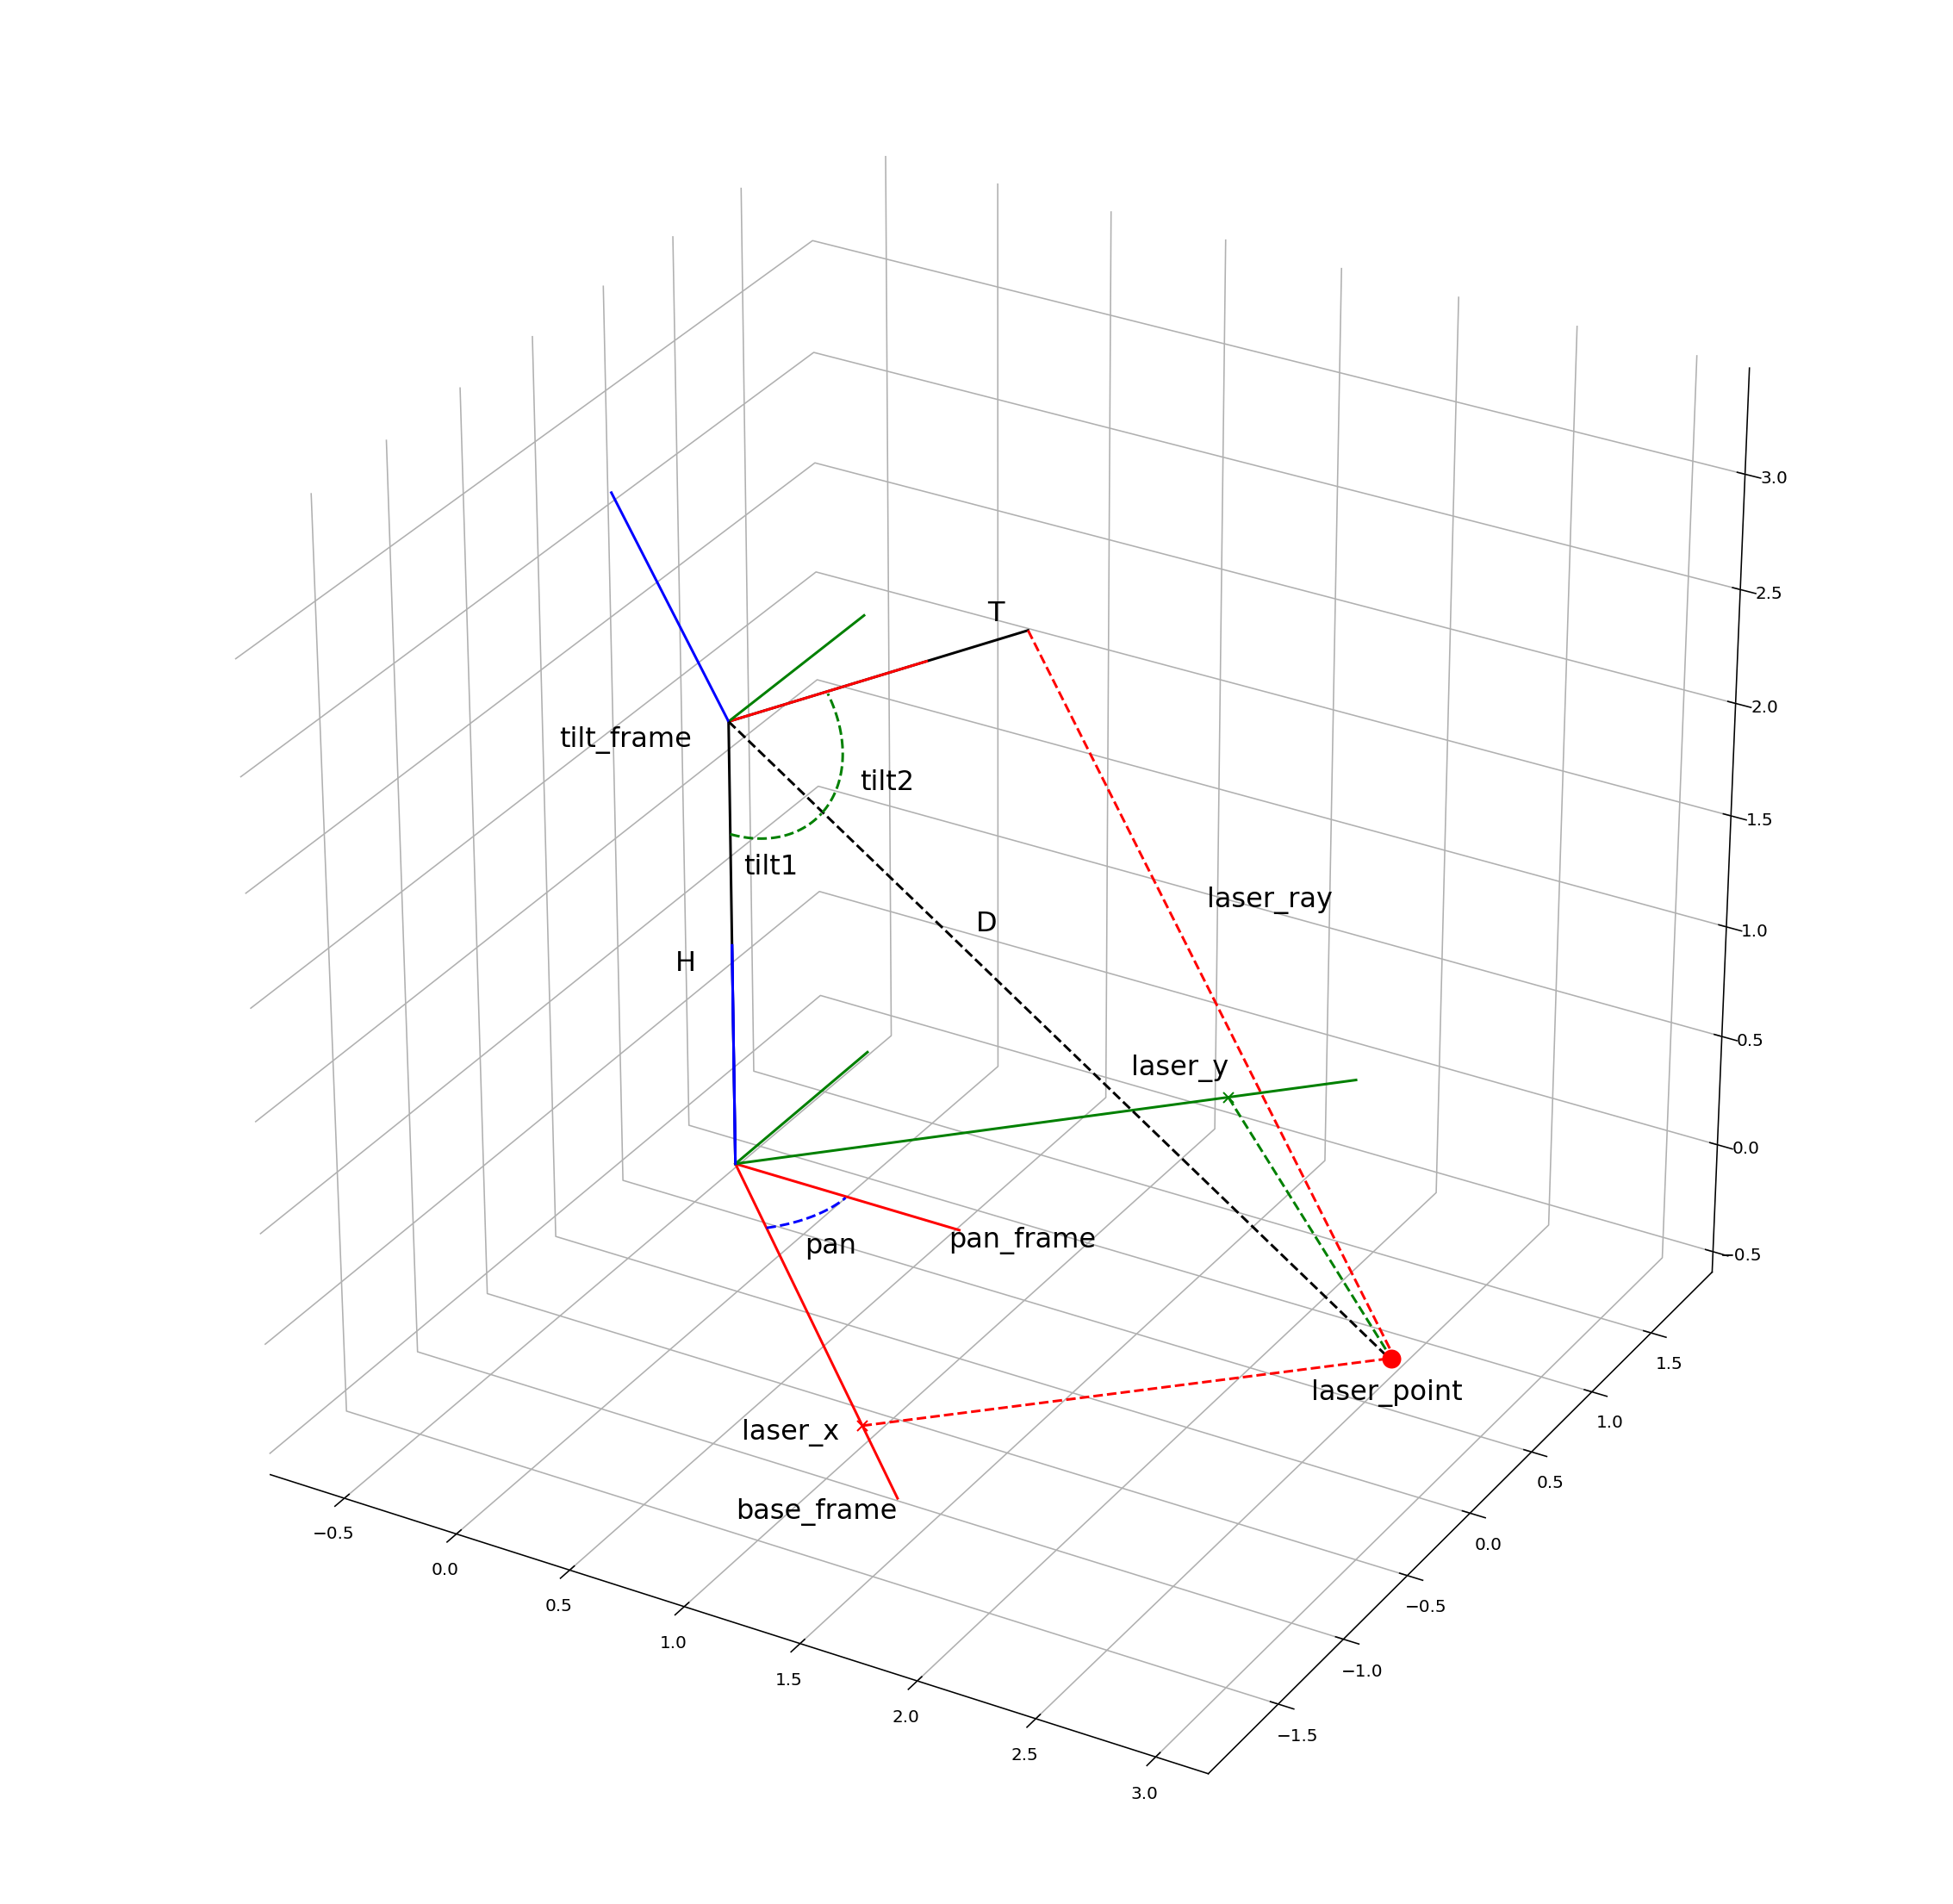
\includegraphics[width=\textwidth]{img/model2XY.png}%
	\caption{Second Model, Pan \& Tilt}
	\label{fig:secondModelPanTilt}
\end{figure}
First, we recall \textbf{L}, \textbf{D} and we introduce \textbf{T}:
\begin{itemize}
    \item \textbf{L} as the distance from the \textbf{pan\_frame} origin to the projection of the laser point on the \textbf{base\_frame};
    \item \textbf{D} as the distance from the \textbf{tilt\_frame} origin to the laser point;
    \item \textbf{T} as the known distance from the \textbf{tilt\_frame} origin to the laser ray origin.
\end{itemize}
As we can see in figure \ref{fig:secondModelPanTilt}, we have to decompose \textbf{tilt} in two parts, this is why we explicitly draw \textbf{D} that time. On the contrary, \textbf{pan} is obtained in the same way we did for the first model, thus:
\begin{align}
	pan=& \arctan\bigg(\frac{y}{x}\bigg)\label{eq:panik2}
\end{align}
Then we compute \textbf{L} and \textbf{D}:
\begin{align}
	L=& \sqrt{x^2+y^2}\\
	D=& \sqrt{(H-z)^2 + L^2}
\end{align}
Finally,
\begin{align}
	tilt1 =& \arcatn\bigg(\frac{L}{H-z}\bigg)\\
	tilt2 =& \arctan\bigg(\frac{D}{T}\bigg)\\
	tilt =& tilt1 + tilt2
\end{align}

\\
